\documentclass[14pt]{extbook}
\usepackage{multicol, enumerate, enumitem, hyperref, color, soul, setspace, parskip, fancyhdr} %General Packages
\usepackage{amssymb, amsthm, amsmath, bbm, latexsym, units, mathtools} %Math Packages
\everymath{\displaystyle} %All math in Display Style
% Packages with additional options
\usepackage[headsep=0.5cm,headheight=12pt, left=1 in,right= 1 in,top= 1 in,bottom= 1 in]{geometry}
\usepackage[usenames,dvipsnames]{xcolor}
\usepackage{dashrule}  % Package to use the command below to create lines between items
\newcommand{\litem}[1]{\item#1\hspace*{-1cm}\rule{\textwidth}{0.4pt}}
\pagestyle{fancy}
\lhead{FinalExam}
\chead{}
\rhead{Version A}
\lfoot{4952-8460}
\cfoot{}
\rfoot{Makeup Early Exam}
\begin{document}

\begin{enumerate}
\litem{
Construct the lowest-degree polynomial given the zeros below. Then, choose the intervals that contain the coefficients of the polynomial in the form $ax^3+bx^2+cx+d$.\[ 4, \frac{2}{3}, \text{ and } \frac{1}{4} \]\begin{enumerate}[label=\Alph*.]
\item \( a \in [11, 20], b \in [-64, -52], c \in [37, 51], \text{ and } d \in [6, 12] \)
\item \( a \in [11, 20], b \in [35, 42], c \in [-48, -34], \text{ and } d \in [6, 12] \)
\item \( a \in [11, 20], b \in [57, 67], c \in [37, 51], \text{ and } d \in [6, 12] \)
\item \( a \in [11, 20], b \in [-64, -52], c \in [37, 51], \text{ and } d \in [-11, -6] \)
\item \( a \in [11, 20], b \in [51, 57], c \in [16, 20], \text{ and } d \in [-11, -6] \)

\end{enumerate} }
\litem{
Choose the graph of the equation below.\[ f(x) = \sqrt{x + 10} + 3 \]\begin{enumerate}[label=\Alph*.]
\begin{multicols}{2}\item 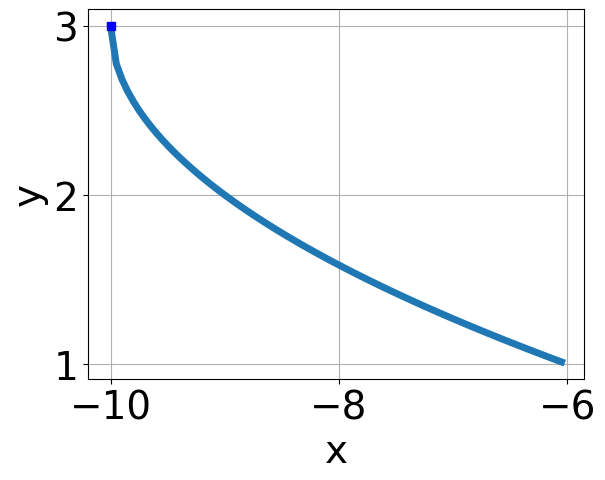
\includegraphics[width = 0.3\textwidth]{../Figures/radicalEquationToGraphAA.png}\item 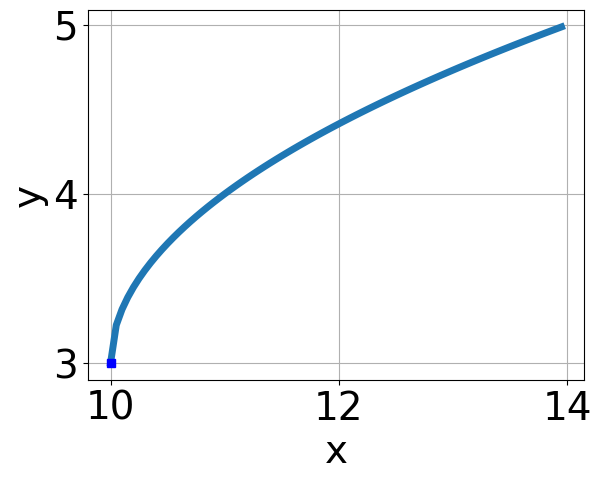
\includegraphics[width = 0.3\textwidth]{../Figures/radicalEquationToGraphBA.png}\item 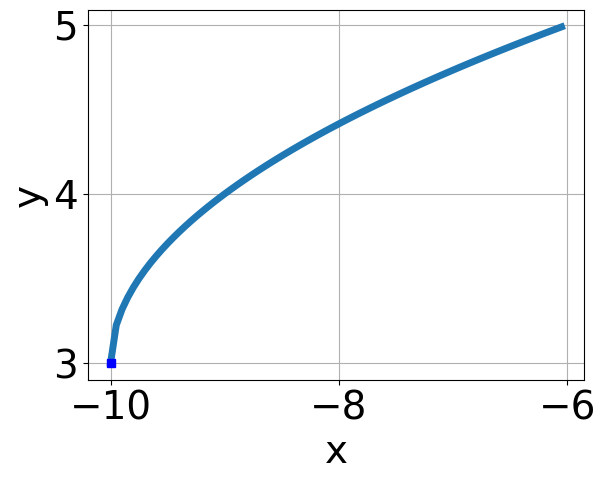
\includegraphics[width = 0.3\textwidth]{../Figures/radicalEquationToGraphCA.png}\item 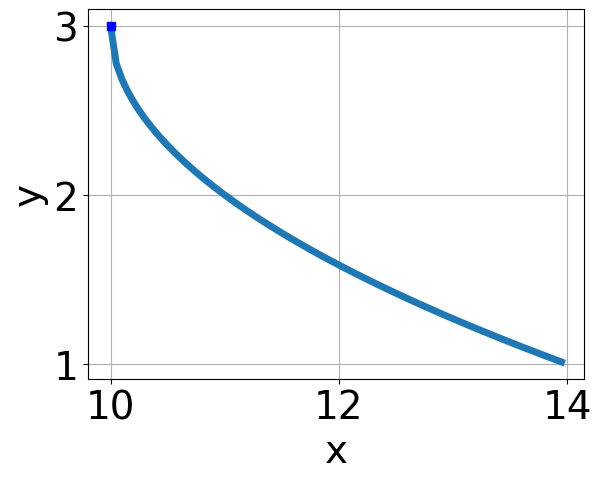
\includegraphics[width = 0.3\textwidth]{../Figures/radicalEquationToGraphDA.png}\end{multicols}\item None of the above.
\end{enumerate} }
\litem{
Which of the following equations \textit{could} be of the graph presented below?
\begin{center}
    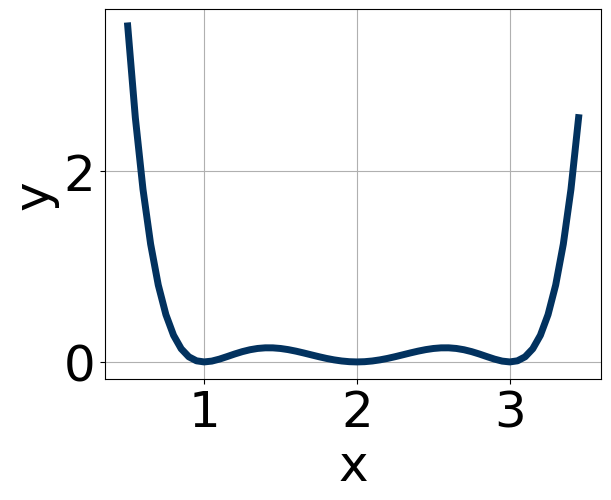
\includegraphics[width=0.5\textwidth]{../Figures/polyGraphToFunctionA.png}
\end{center}
\begin{enumerate}[label=\Alph*.]
\item \( 17(x - 2)^{8} (x - 1)^{6} (x - 3)^{6} \)
\item \( 13(x - 2)^{8} (x - 1)^{11} (x - 3)^{7} \)
\item \( 15(x - 2)^{4} (x - 1)^{4} (x - 3)^{9} \)
\item \( -15(x - 2)^{10} (x - 1)^{10} (x - 3)^{4} \)
\item \( -16(x - 2)^{4} (x - 1)^{6} (x - 3)^{11} \)

\end{enumerate} }
\litem{
Solve the radical equation below. Then, choose the interval(s) that the solution(s) belongs to.\[ \sqrt{-6 x - 5} - \sqrt{7 x - 9} = 0 \]\begin{enumerate}[label=\Alph*.]
\item \( \text{All solutions lead to invalid or complex values in the equation.} \)
\item \( x_1 \in [-0.85, -0.54] \text{ and } x_2 \in [-0.33,0.51] \)
\item \( x \in [0.17,0.34] \)
\item \( x_1 \in [-0.85, -0.54] \text{ and } x_2 \in [1.21,1.84] \)
\item \( x \in [-1.11,-0.91] \)

\end{enumerate} }
\litem{
Solve the quadratic equation below. Then, choose the intervals that the solutions belong to, with $x_1 \leq x_2$ (if they exist).\[ -17x^{2} +15 x + 9 = 0 \]\begin{enumerate}[label=\Alph*.]
\item \( x_1 \in [-0.55, -0.04] \text{ and } x_2 \in [1.12, 1.4] \)
\item \( x_1 \in [-2.02, -0.96] \text{ and } x_2 \in [-0.21, 0.68] \)
\item \( x_1 \in [-22.28, -21.92] \text{ and } x_2 \in [6.79, 7.2] \)
\item \( x_1 \in [-29.75, -28.12] \text{ and } x_2 \in [29.32, 29.49] \)
\item \( \text{There are no Real solutions.} \)

\end{enumerate} }
\litem{
Graph the equation below.\[ f(x) = (x+2)^2 - 17 \]\begin{enumerate}[label=\Alph*.]
\begin{multicols}{2}\item 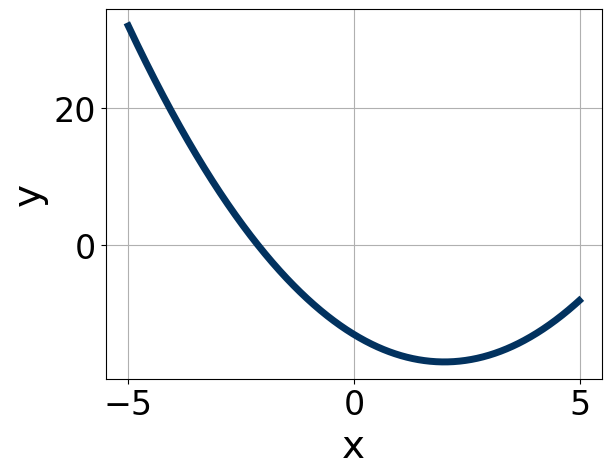
\includegraphics[width = 0.3\textwidth]{../Figures/quadraticEquationToGraphAA.png}\item 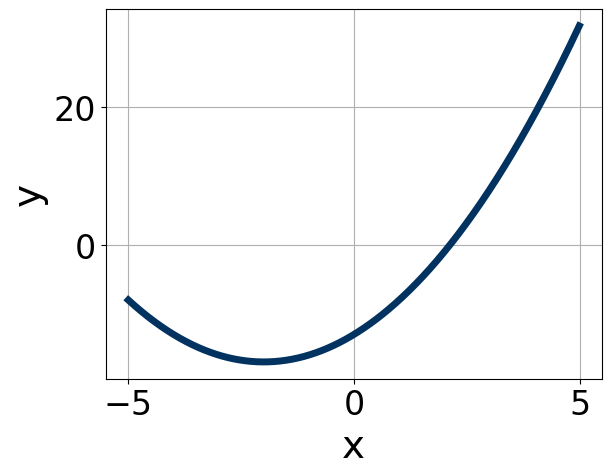
\includegraphics[width = 0.3\textwidth]{../Figures/quadraticEquationToGraphBA.png}\item 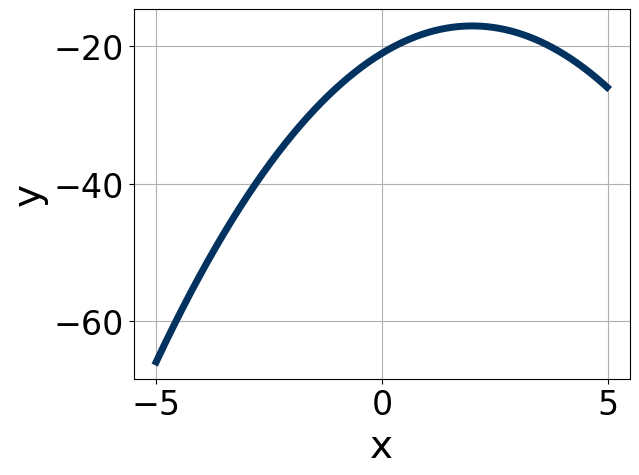
\includegraphics[width = 0.3\textwidth]{../Figures/quadraticEquationToGraphCA.png}\item 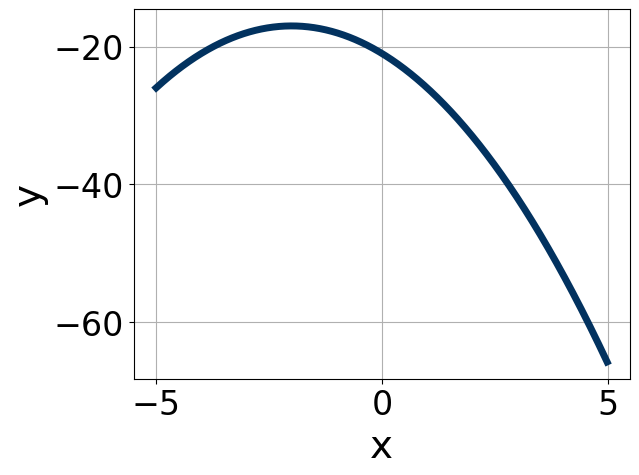
\includegraphics[width = 0.3\textwidth]{../Figures/quadraticEquationToGraphDA.png}\end{multicols}\item None of the above.
\end{enumerate} }
\litem{
Find the equation of the line described below. Write the linear equation as $ y=mx+b $ and choose the intervals that contain $m$ and $b$.\[ \text{Perpendicular to } 5 x - 9 y = 13 \text{ and passing through the point } (4, 8). \]\begin{enumerate}[label=\Alph*.]
\item \( m \in [-3.2, -1.5] \hspace*{3mm} b \in [10.2, 17.2] \)
\item \( m \in [-0.9, 0.5] \hspace*{3mm} b \in [10.2, 17.2] \)
\item \( m \in [1, 2.1] \hspace*{3mm} b \in [-3.2, 2.8] \)
\item \( m \in [-3.2, -1.5] \hspace*{3mm} b \in [-15.2, -14.2] \)
\item \( m \in [-3.2, -1.5] \hspace*{3mm} b \in [2, 6] \)

\end{enumerate} }
\litem{
What is the domain of the function below?\[ f(x) = \sqrt[7]{-7 x + 8} \]\begin{enumerate}[label=\Alph*.]
\item \( \text{The domain is } (-\infty, a], \text{   where } a \in [0.44, 1.05] \)
\item \( \text{The domain is } [a, \infty), \text{   where } a \in [0.86, 1] \)
\item \( \text{The domain is } [a, \infty), \text{   where } a \in [0.93, 2.03] \)
\item \( \text{The domain is } (-\infty, a], \text{   where } a \in [0.88, 1.46] \)
\item \( (-\infty, \infty) \)

\end{enumerate} }
\litem{
Write the equation of the graph presented below in the form $f(x)=ax^2+bx+c$, assuming  $a=1$ or $a=-1$. Then, choose the intervals that $a, b,$ and $c$ belong to.
\begin{center}
    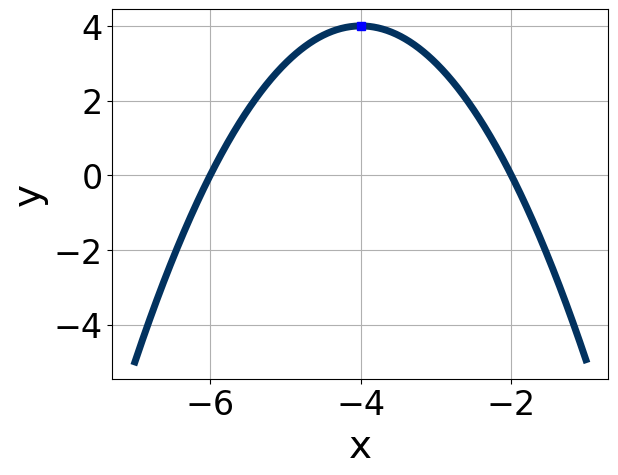
\includegraphics[width=0.5\textwidth]{../Figures/quadraticGraphToEquationA.png}
\end{center}
\begin{enumerate}[label=\Alph*.]
\item \( a \in [-0.6, 1.1], \hspace*{5mm} b \in [4, 13], \text{ and } \hspace*{5mm} c \in [16, 25] \)
\item \( a \in [-2.9, 0.7], \hspace*{5mm} b \in [-10, -7], \text{ and } \hspace*{5mm} c \in [-12, -8] \)
\item \( a \in [-2.9, 0.7], \hspace*{5mm} b \in [4, 13], \text{ and } \hspace*{5mm} c \in [-12, -8] \)
\item \( a \in [-2.9, 0.7], \hspace*{5mm} b \in [4, 13], \text{ and } \hspace*{5mm} c \in [-20, -18] \)
\item \( a \in [-0.6, 1.1], \hspace*{5mm} b \in [-10, -7], \text{ and } \hspace*{5mm} c \in [16, 25] \)

\end{enumerate} }
\litem{
Which of the following intervals describes the Range of the function below?\[ f(x) = -\log_2{(x-4)}-8 \]\begin{enumerate}[label=\Alph*.]
\item \( (-\infty, a), a \in [7, 14] \)
\item \( [a, \infty), a \in [-4, 3] \)
\item \( (-\infty, a), a \in [-13, -7] \)
\item \( [a, \infty), a \in [-2, 7] \)
\item \( (-\infty, \infty) \)

\end{enumerate} }
\litem{
Choose the equation of the function graphed below.
\begin{center}
    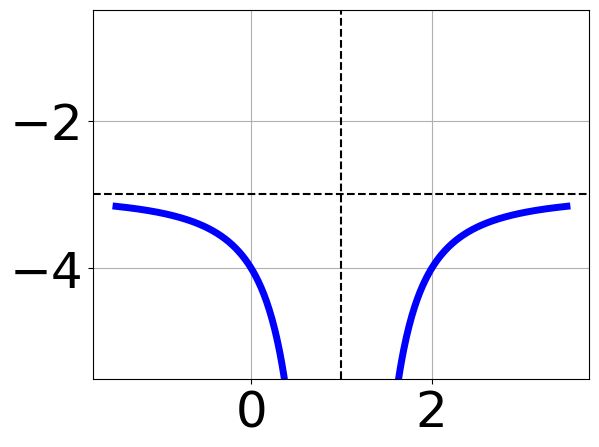
\includegraphics[width=0.5\textwidth]{../Figures/rationalGraphToEquationA.png}
\end{center}
\begin{enumerate}[label=\Alph*.]
\item \( f(x) = \frac{-1}{x + 1} - 3 \)
\item \( f(x) = \frac{1}{x - 1} - 3 \)
\item \( f(x) = \frac{1}{(x - 1)^2} - 3 \)
\item \( f(x) = \frac{-1}{(x + 1)^2} - 3 \)
\item \( \text{None of the above} \)

\end{enumerate} }
\litem{
Choose the \textbf{smallest} set of Real numbers that the number below belongs to.\[ -\sqrt{\frac{576}{625}} \]\begin{enumerate}[label=\Alph*.]
\item \( \text{Rational} \)
\item \( \text{Whole} \)
\item \( \text{Not a Real number} \)
\item \( \text{Integer} \)
\item \( \text{Irrational} \)

\end{enumerate} }
\litem{
Solve the linear equation below. Then, choose the interval that contains the solution.\[ \frac{-9x + 9}{8} - \frac{-9x -6}{4} = \frac{9x + 8}{5} \]\begin{enumerate}[label=\Alph*.]
\item \( x \in [9.1, 11.7] \)
\item \( x \in [-0.5, 0.6] \)
\item \( x \in [0.6, 3.8] \)
\item \( x \in [-5.9, -2.2] \)
\item \( \text{There are no real solutions.} \)

\end{enumerate} }
\litem{
Describe the zero behavior of the zero $x = 4$ of the polynomial below.\[ f(x) = -5(x + 4)^{8}(x - 4)^{9}(x + 9)^{4}(x - 9)^{5} \]\begin{enumerate}[label=\Alph*.]
\begin{multicols}{2}\item 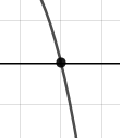
\includegraphics[width = 0.3\textwidth]{../Figures/polyZeroBehaviorAA.png}\item 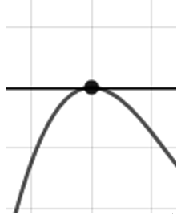
\includegraphics[width = 0.3\textwidth]{../Figures/polyZeroBehaviorBA.png}\item 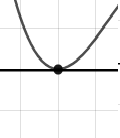
\includegraphics[width = 0.3\textwidth]{../Figures/polyZeroBehaviorCA.png}\item 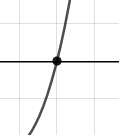
\includegraphics[width = 0.3\textwidth]{../Figures/polyZeroBehaviorDA.png}\end{multicols}\item None of the above.
\end{enumerate} }
\litem{
Solve the linear inequality below. Then, choose the constant and interval combination that describes the solution set.\[ -6x + 4 \geq 7x -3 \]\begin{enumerate}[label=\Alph*.]
\item \( [a, \infty), \text{ where } a \in [-1.35, -0.39] \)
\item \( (-\infty, a], \text{ where } a \in [-0.23, 1.19] \)
\item \( [a, \infty), \text{ where } a \in [0.37, 2.04] \)
\item \( (-\infty, a], \text{ where } a \in [-1.81, 0.13] \)
\item \( \text{None of the above}. \)

\end{enumerate} }
\litem{
Simplify the expression below and choose the interval the simplification is contained within.\[ 2 - 12^2 + 4 \div 8 * 10 \div 3 \]\begin{enumerate}[label=\Alph*.]
\item \( [-142.6, -140.45] \)
\item \( [-141.71, -139.39] \)
\item \( [147.49, 149.13] \)
\item \( [145.93, 146.22] \)
\item \( \text{None of the above} \)

\end{enumerate} }
\litem{
Solve the linear inequality below. Then, choose the constant and interval combination that describes the solution set.\[ \frac{-10}{3} - \frac{7}{7} x > \frac{-4}{9} x - \frac{5}{2} \]\begin{enumerate}[label=\Alph*.]
\item \( (-\infty, a), \text{ where } a \in [-2.5, 0.5] \)
\item \( (-\infty, a), \text{ where } a \in [1.5, 3.5] \)
\item \( (a, \infty), \text{ where } a \in [0.5, 3.5] \)
\item \( (a, \infty), \text{ where } a \in [-1.5, 0.5] \)
\item \( \text{None of the above}. \)

\end{enumerate} }
\litem{
Solve the rational equation below. Then, choose the interval(s) that the solution(s) belongs to.\[ \frac{-7x}{-6x + 6} + \frac{-7x^{2}}{36x^{2} -72 x + 36} = \frac{2}{-6x + 6} \]\begin{enumerate}[label=\Alph*.]
\item \( x \in [1.12,1.42] \)
\item \( x_1 \in [-0.37, -0.13] \text{ and } x_2 \in [0.86,1.01] \)
\item \( x \in [0.92,1.03] \)
\item \( x_1 \in [-0.37, -0.13] \text{ and } x_2 \in [1.13,1.46] \)
\item \( \text{All solutions lead to invalid or complex values in the equation.} \)

\end{enumerate} }
\litem{
Simplify the expression below into the form $a+bi$. Then, choose the intervals that $a$ and $b$ belong to.\[ \frac{36 + 66 i}{5 - 3 i} \]\begin{enumerate}[label=\Alph*.]
\item \( a \in [-19, -17.5] \text{ and } b \in [12.5, 14] \)
\item \( a \in [-1, 0] \text{ and } b \in [437.5, 438.5] \)
\item \( a \in [-1, 0] \text{ and } b \in [12.5, 14] \)
\item \( a \in [6.5, 8.5] \text{ and } b \in [-22.5, -21.5] \)
\item \( a \in [10.5, 12.5] \text{ and } b \in [6, 7.5] \)

\end{enumerate} }
\litem{
Solve the rational equation below. Then, choose the interval(s) that the solution(s) belongs to.\[ \frac{6}{-7x + 6} + -9 = \frac{-3}{56x -48} \]\begin{enumerate}[label=\Alph*.]
\item \( x_1 \in [0.6, 0.72] \text{ and } x_2 \in [-0.23,1.77] \)
\item \( x_1 \in [-1.02, -0.9] \text{ and } x_2 \in [-0.23,1.77] \)
\item \( \text{All solutions lead to invalid or complex values in the equation.} \)
\item \( x \in [-1.02,-0.9] \)
\item \( x \in [0.77,3.77] \)

\end{enumerate} }
\litem{
Solve the equation for $x$ and choose the interval that contains the solution (if it exists).\[ 3^{5x+3} = 16^{3x-4} \]\begin{enumerate}[label=\Alph*.]
\item \( x \in [3.09, 6.09] \)
\item \( x \in [-0.52, 4.48] \)
\item \( x \in [-4.5, -0.5] \)
\item \( x \in [-10.19, -6.19] \)
\item \( \text{There is no Real solution to the equation.} \)

\end{enumerate} }
\litem{
Which of the following intervals describes the Range of the function below?\[ f(x) = e^{x-1}-8 \]\begin{enumerate}[label=\Alph*.]
\item \( (a, \infty), a \in [-11, -7] \)
\item \( [a, \infty), a \in [-11, -7] \)
\item \( (-\infty, a], a \in [8, 11] \)
\item \( (-\infty, a), a \in [8, 11] \)
\item \( (-\infty, \infty) \)

\end{enumerate} }
\litem{
First, find the equation of the line containing the two points below. Then, write the equation as $ y=mx+b $ and choose the intervals that contain $m$ and $b$.\[ (-7, 11) \text{ and } (9, 3) \]\begin{enumerate}[label=\Alph*.]
\item \( m \in [-1.2, -0.2] \hspace*{3mm} b \in [-7, -2] \)
\item \( m \in [-1.2, -0.2] \hspace*{3mm} b \in [17, 22] \)
\item \( m \in [-1.2, -0.2] \hspace*{3mm} b \in [-7.5, -6.5] \)
\item \( m \in [-1.2, -0.2] \hspace*{3mm} b \in [5.5, 9.5] \)
\item \( m \in [-0.4, 3.2] \hspace*{3mm} b \in [-3.5, 6.5] \)

\end{enumerate} }
\litem{
Solve the linear inequality below. Then, choose the constant and interval combination that describes the solution set.\[ -6 + 7 x < \frac{33 x - 3}{4} \leq -3 + 6 x \]\begin{enumerate}[label=\Alph*.]
\item \( (-\infty, a] \cup (b, \infty), \text{ where } a \in [-4.2, -3.2] \text{ and } b \in [-2.6, -0.1] \)
\item \( (a, b], \text{ where } a \in [-6.2, -1.2] \text{ and } b \in [-1.7, -0.7] \)
\item \( [a, b), \text{ where } a \in [-4.2, -3.2] \text{ and } b \in [-4, 0] \)
\item \( (-\infty, a) \cup [b, \infty), \text{ where } a \in [-4.2, -0.2] \text{ and } b \in [-1, 0] \)
\item \( \text{None of the above.} \)

\end{enumerate} }
\end{enumerate}

\end{document}